\documentclass[main]{subfiles}

\begin{document}

\section{Лекция 5}

Научимся работать с множествами всех классов гомотопности. Начнем с тривиальных примеров:
\begin{itemize}
	\item $ \Abs{\pi(T, \Emp)} = 0 $ при $ T \neq \Emp $;
	\item $ \Abs{\pi(\Emp, T)} = 1 $, так как принято считать, что для любого множества $ A $ существует
		единственое отображение $ \Emp \colon \Emp \to A $.
\end{itemize}
Это можно понять, вспомнив формальное определение отображения $ f \colon A \to B $
(как множество $ f \ssq A \times B $, где для любого $ a \in A $ существует единственная пара $ (a, b) \in f $).

\begin{remark}
	Хотя мы формально определяли топологические пространства только для непустых множеств, этот пример все равно
	полезен для понимания.
\end{remark}

Рассмотрим теперь топологическое пространство $ A \ssq \R^n $, где $ A $ --- выпуклое множество.
Каким может быть $ \pi(T, A) $?
\begin{itemize}
	\item Начнем с простого случая: $ \Abs{\pi(\pt, A)} = 1 $, где $ \pt $ --- одноточечное топологическое пространство
		(это стандартное обозначение). Действительно, все отображения по сути <<ставят точку>>
		во множестве A. Ясно, что их легко стянуть в одну конкретную (здесь важна выпуклость), так что все отображения
		друг другу гомотопны.
	\item Однако такие же рассуждения справедливы и для произвольного пространства $ T $. Пусть
		$ f_1, f_2 \colon T \to A $. Тогда гомотопией между ними будет отображения
		$ F \colon T \times [0; 1] \to A $, определенное следующим образом: для $ x \in T $ и
		$ t \in [0; 1] $ положим $ F(x, t) = (f_1 + (f_2 - f_1) t)(x) $. Каждый раз этот элемент лежит
		во множестве $ A $ в силу его выпоклости. Можно доказать, что это отображение непрерывно.
\end{itemize}

\begin{theorem}
	Пусть $ T_1 $, $ T_2 $ --- топологические пространства, $ t \in T_2 $. Тогда если для отображения
	$ f \colon T_1 \to T_2 $ верно $ f(T_1) = \Set{t} $, то отображение $ f $ непрерывно.
\end{theorem}

\begin{proof}
	Действительно, для любого открытого множества $ V \in \W_2 $ верно
		\[ f^{-1}(V) = \left. \begin{cases}
				\Emp, & \text{если } t \notin V; \\
				T_1, & \text{если } t \in V
			\end{cases} \right\} \in \W_1.
		\]
\end{proof}

Вернемся теперь к фундаментальным группам.

\FactorSetIsGroup

\begin{restatable}[из домашнего задания]{exercise}{ExcXIII}
	Докажите существование нейтрального элемента. В качестве $ e $ возьмите петлю $ e \colon t \mapsto x_0 $. Тогда
	класс эквивалентности этой петли будет нейтральным элементом в группе, то есть для любой петли $ a $ верно
	$ [a][e] = [e][a] = [a] $.
\end{restatable}

\begin{restatable}[из домашнего задания]{exercise}{ExcXIV}
	Докажите существование обратного элемента. Для каждой петли $ a $ рассмотрите петлю
	$ a^{-1} \colon t \mapsto a(1 - t) $. Тогда для $ [a] $ обратным элементом будет элемент $ [a^{-1}] $, то есть
	$ [a][a^{-1}] = [a^{-1}][a] = [e] $. Кроме того, нужно обосновать корректность: если $ b \sim a $, то
	$ [a][b^{-1}] = [b^{-1}][a] = [e] $.
\end{restatable}

\begin{proof} \leavevmode
	\begin{phased}
		\item[Корректность.] Покажем, что если $ a_1 \sim a_2 $, то для любой петли $ b $ верно $ [b a_1] = [b a_2] $,
			то есть $ b a_1 \sim b a_2 $. Построим гомотопию между ними. Определим $ C \colon [0; 1]^2 \to X $
			следующим образом: для любых $ t \in [0; 1] $ и $ \tau \in [0; 1] $ положим
				\[ C(t, \tau) = \begin{cases}
						A(2 t, \tau), & \text{если } t \in \left[ 0; \frac{1}{2} \right]; \\
						b(2 t - 1), & \text{если } t \in \left[ \frac{1}{2}; 1 \right],
					\end{cases}
				\]
			где $ A \colon [0; 1]^2 \to X $ --- гомотопия между $ a_1 $, $ a_2 $. Тогда отображение $ C $ корректно
			определено при $ t = \frac{1}{2} $. При $ \tau = 0 $ оно совпадает с $ b a_1 $, а при $ \tau = 1 $ ---
			с $ b a_2 $. Непрерывность следует из того, что на $ \left[0; \frac{1}{2}\right] \times [0; 1] $ это
			композиция непрерывных отображений $ A $ и линейного преобразования пары координат, а на
			$ \left[ \frac{1}{2}; 1 \right] \times [0; 1] $ это непрерывное отображение $ b $.
			\begin{remark}
				Удобно представлять гомотопию на квадрате с координатами $ t \times \tau $: на левой половине
				проходится гомотопия $ A $, а на правой --- сама петля $ b $. Более того, по картинке проще понимать
				непрерывность, поскольку область определения явным образом разбита на замкнутые части.
			\end{remark}
			\begin{figure}[H]
				\centering 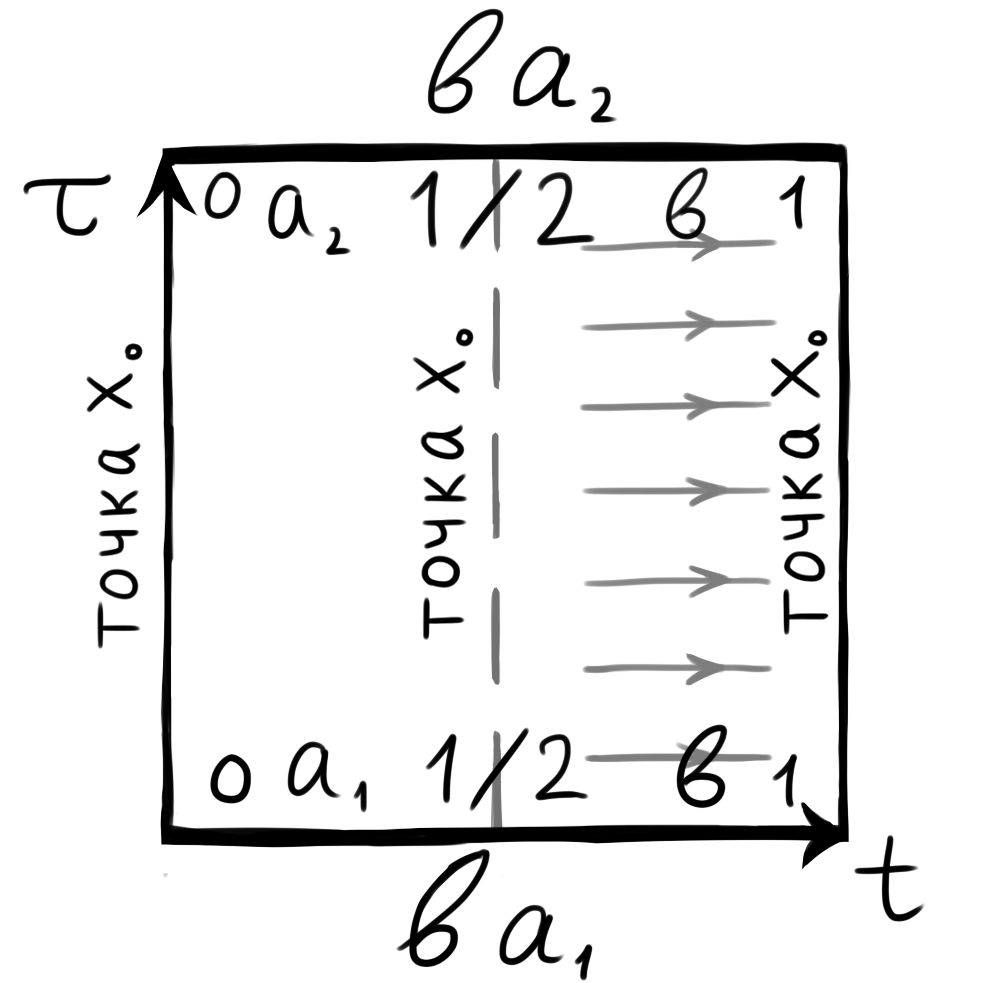
\includegraphics[width=0.5\textwidth]{homotopy-plain-1}
			\end{figure}
		\item[Ассоциативность.] Пусть $ [a], [b], [c] \in \pi_1(X, x_0) $. Тогда по определнию операции на множестве
			$ ([a][b])[c] = [(ab)c] $ и $ [a]([b][c]) = [a(bc)] $, так что достаточно доказать $ (ab)c \sim a(bc) $.
			Воспользуемся картинкой и запишем уравнение гомотопии между данными петлями:
			\begin{figure}[H]
				\centering 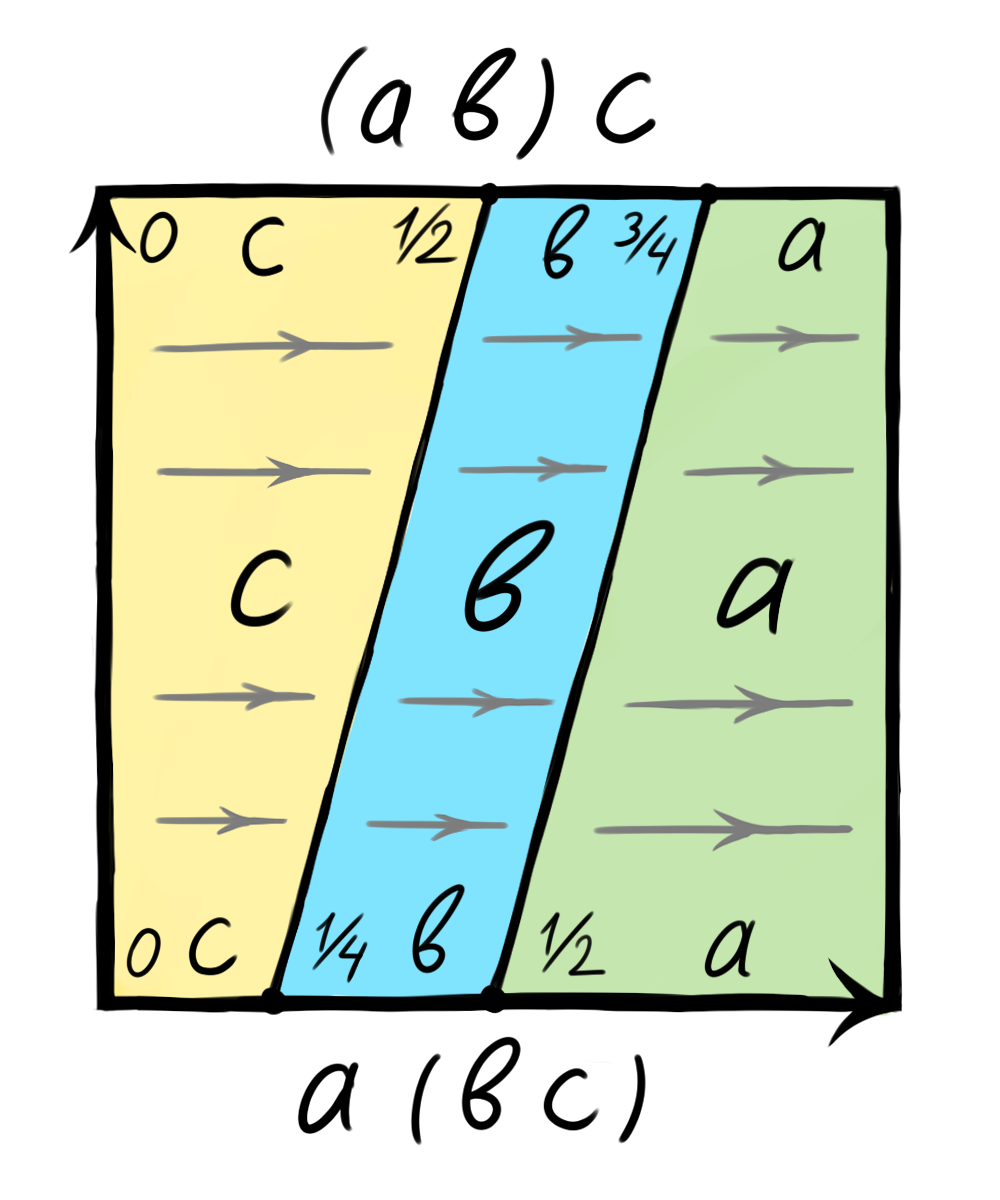
\includegraphics[width=0.5\textwidth]{associativity}
			\end{figure}
				\[ F(t, \tau) = \begin{cases}
						c\left(\frac{4 t}{1 + \tau}\right),
							& \text{если } \tau \Gr 4 t - 1 \text{ и } (t, \tau) \in [0; 1]^2; \\
						b(4 t - 1 - \tau),
							& \text{если } 4 t - 1 \Le \tau \Le 4 t - 2 \text{ и } (t, \tau) \in [0; 1]^2; \\
						a\left(\frac{4 t - 4}{2 - \tau} +1\right),
							& \text{если } \tau \Le 4 t - 2 \text{ и } (t, \tau) \in [0; 1]^2.
					\end{cases}
				\]
			Стандартным образом доказывается непрерывность этого отображения.
	\end{phased}
\end{proof}

\subsection{Фундаментальная группа окружности}

\begin{remark}
	Напомним, отображением $ f_k $, где $ k \in \Z $, называется отображение окружности в окружность, заданное
	формулой: для $ t \in [0; 1] $ выполнено $ f_k( e^{2 \pi i t}) = e^{2 \pi i k t} $.
\end{remark}

В ближайшее время мы будем стремиться к доказательству следующих двух предложений.

\begin{proposition*}
	Пусть $ k_1, k_2 \in \Z $ и $ k_1 \neq k_2 $. Тогда $ f_{k_1} \not \sim f_{k_2} $.
\end{proposition*}

\begin{proposition*}
	Любая петля $ \phi \colon ([0; 1], \Set{0, 1}) \to (\S^1, \Set{0})$ гомотопна одну из отображений $ f_k $, где
	$ k \in \Z $.
\end{proposition*}

\begin{remark}
	Часто мы будем считать, что $ \S^1 = \Set{ z \in \C \mid \Abs{z} = 1 } $, а параметризуем эту окружность
	параметром $ t \in [0; 1] $, так что <<точке>> $ t \in [0; 1] $ соответствует точка $ e^{2 \pi i t} $.
\end{remark}

\begin{remark}
	Если петля $ \phi \colon ([0; 1], \Set{0, 1}) \to (\S^1, \Set{0})$ гомотопна отображению $ f_k $ при $ k \in \Z $,
	то число $ k $ называется индексом петли $ \phi $ и обозначается $ \Ind(\phi) $. Однако мы определим это понятие
	по-другому, через поднятия, поскольку предложенное определение неудобно для доказательства основной теоремы:
	$ \pi_1(\S^1, 0) \simeq \Z $.
\end{remark}

\begin{definition}
	\emph{Накрытием $ p \colon \R \to \S^1 $} называется отображение, заданное формулой: для $ t \in \R $ выполнено
	$ p(t) = e^{2 \pi i t} $.
\end{definition}

\begin{definition}
	Пусть $ f \colon ([0; 1], \Set{0}) \to (\S^1, \Set{0}) $ --- некоторый непрерывный пусть на окружности.
	Тогда \emph{поднятием пути $ f $} называется такое отображение
	$ \Up{f} \colon ([0; 1], \Set{0}) \to (\R, \Set{0}) $, что $ f = p \circ \Up{f} $.
\end{definition}

\begin{restatable}{lemma}{LiftExists}
	Для люого непрерывного пути $ f \colon ([0; 1], \Set{0}) \to (\S^1, \Set{0}) $ на окружности существует и
	единственно поднятие $ \Up{f} \colon ([0; 1], \Set{0}) \to (\R, \Set{0}) $.
\end{restatable}

Покажем, как эту лемму можно использовать. Докажем мы ее в следующий раз.

\begin{definition}
	\emph{Индексом петли} $ a $ называется число $ \Ind(a) = \Up{a}(1) $.
\end{definition}

\begin{statement}
	Для любой петли $ a $ ее индекс $ \Ind(a) $ целый.
\end{statement}

\begin{proof}
	Так как $ a = p \circ \Up{a} $ и $ a(1) = 0 $, то $ \Up{a}(1) \in p^{-1}(0) $. Но заметим, что
		\[ p(t) = 0 \quad \iaoi \quad e^{2 \pi i t} = 0 \quad \iaoi \quad t \in \Z. \]
	Таким образом, $ \Ind(a) = \Up{a}(1) \in \Z $.
\end{proof}

\begin{statement}
	$ \Ind(f_k) = k $.
\end{statement}

\begin{proof}
	Заметим, что для любого $ t \in [0; 1] $ верно $ \Up{f_k}(t) = k t $. Действительно, в этом случае
	$ f_k(e^{2 \pi i t}) = e^{2 \pi i \Up{f_k}(t)} $. Тогда в силу единственности поднятия корректно определено число
	$ \Ind(f_k) = k $.
\end{proof}

\end{document}
